% This file was created by matlab2tikz.
%
%The latest updates can be retrieved from
%  http://www.mathworks.com/matlabcentral/fileexchange/22022-matlab2tikz-matlab2tikz
%where you can also make suggestions and rate matlab2tikz.
%
\definecolor{mycolor1}{rgb}{0.77600,0.15600,0.15600}%
%
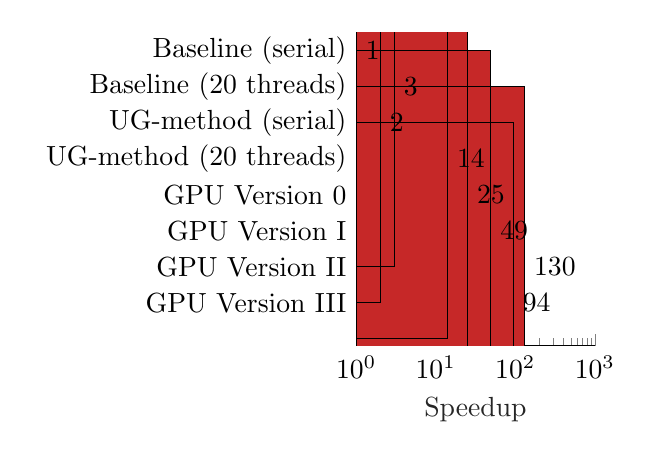
\begin{tikzpicture}

\begin{axis}[%
width=0.25\textwidth,
height=1.566in,
at={(1.637in,0.481in)},
scale only axis,
bar shift auto,
log origin=infty,
xmode=log,
xmin=1,
xmax=1000,
xminorticks=true,
xlabel style={font=\color{white!15!black}},
xlabel={Speedup},
ymin=-0.2,
ymax=8.5,
ytick={1,2,3,4,5,6,7,8},
yticklabels={{GPU Version III},{GPU Version II},{GPU Version I},{GPU Version 0},{  UG-method (20 threads)},{UG-method (serial)},{Baseline (20 threads)}, {Baseline (serial)}},
axis background/.style={fill=white},
axis x line*=bottom,
axis y line*=left
]
\addplot[xbar, bar width=10, fill=mycolor1, draw=black, area legend] table[row sep=crcr] {%
94	1\\
130	2\\
49	3\\
25	4\\
14	5\\
2	6\\
3	7\\
1	8\\
};
\node[right, align=left]
at (axis cs:94,1) { 94};
\node[right, align=left]
at (axis cs:130,2) {130};
\node[right, align=left]
at (axis cs:49,3) { 49};
\node[right, align=left]
at (axis cs:25,4) { 25};
\node[right, align=left]
at (axis cs:14,5) { 14};
\node[right, align=left]
at (axis cs:2,6) {  2};
\node[right, align=left]
at (axis cs:3,7) {  3};
\node[right, align=left]
at (axis cs:1,8) {  1};
\end{axis}
\end{tikzpicture}%